%%
%% This is the merged file using the ACM Sigconf template
%%
\documentclass[sigconf,nonacm]{acmart}

%% ------------------------------------------------------------------------
%% RIGHTS MANAGEMENT INFORMATION
%% ------------------------------------------------------------------------
\setcopyright{none}
\settopmatter{printacmref=false}
\copyrightyear{2026}
\acmYear{2026}
\acmDOI{}

%% Conference information
\acmConference[CS-559 Project]{CS-559 Project}{2025-2026}{Heraklion, Crete}
\acmISBN{}

%% User Packages
\usepackage{graphicx}
\usepackage{textcomp}
\usepackage{xcolor}
\usepackage{booktabs}
\usepackage{multirow}
\usepackage{amsmath}
\usepackage{pgfplots}
\pgfplotsset{compat=1.18}
\definecolor{awsblue}{RGB}{42,104,153}
\definecolor{azureorange}{RGB}{207,132,17}

%% Fix for fancyhdr warning
\setlength{\headheight}{19pt}

\begin{document}

\title{Cross-Platform Performance Evaluation of Serverless Computing\texorpdfstring{\\}{: }A Comparative Study of AWS Lambda and Azure Functions}

%%
%% AUTHORS
%%
\author{Anna Makridou}
\email{csdp1448@csd.uoc.gr}
\affiliation{%
  \institution{University of Crete, Computer Science Department}
  \city{Heraklion}
  \country{Greece}
}

%%
%% ABSTRACT
%%
\begin{abstract}
Serverless computing platforms like AWS Lambda and Azure Functions have gained widespread adoption, yet lack comprehensive performance comparisons using identical code and fair experimental conditions. This course report presents a microbenchmark study comparing AWS Lambda and Azure Functions across seven diverse workloads: four function benchmarks (HTML generation, image processing, file compression, and a custom matrix multiplication benchmark) and three workflow orchestration patterns (sequential, parallel, and map-reduce). Using the SeBS-Flow framework with identical code and inputs, 240 invocations were executed across both platforms, with no recorded failure flags. Results show lower mean Azure benchmark durations in all four cold-flagged and warm-flagged function groups, with 4.6--22.6$\times$ lower cold-flagged benchmark durations and up to 4.9$\times$ faster warm execution for production workloads. For workflows, AWS demonstrates consistent advantages across all three patterns: 10.6$\times$ faster for sequential workflows, 20.8$\times$ faster for parallel execution, and 15.3$\times$ faster for complex map-reduce.
\end{abstract}

%%
%% CCS CONCEPTS
%%
\begin{CCSXML}
<ccs2012>
   <concept>
       <concept_id>10010520.10010521.10010537</concept_id>
       <concept_desc>Computer systems organization~Distributed architectures</concept_desc>
       <concept_significance>500</concept_significance>
   </concept>
   <concept>
       <concept_id>10010520.10010521.10010537.10003100</concept_id>
       <concept_desc>Computer systems organization~Cloud computing</concept_desc>
       <concept_significance>500</concept_significance>
   </concept>
   <concept>
       <concept_id>10003033.10003079.10003080</concept_id>
       <concept_desc>Networks~Network performance evaluation</concept_desc>
       <concept_significance>300</concept_significance>
   </concept>
</ccs2012>
\end{CCSXML}

\ccsdesc[500]{Computer systems organization~Cloud computing}
\ccsdesc[300]{Networks~Network performance evaluation}

%%
%% KEYWORDS
%%
\keywords{Serverless computing, FaaS, AWS Lambda, Azure Functions, Benchmarking, Performance evaluation, Cold starts, Warm Starts, Experiments, Platform Comparison}

%%
%% MAKETITLE
%%
\maketitle

%% ------------------------------------------------------------------------
%% BODY TEXT
%% ------------------------------------------------------------------------

\section{Introduction}

Serverless computing has revolutionized application deployment by abstracting infrastructure management and enabling automatic scaling.

Major cloud providers including Amazon Web Services (AWS Lambda),  Microsoft Azure (Azure Functions) and Google Cloud Platform (GCP Cloud Functions) offer serverless platforms with distinct architectures, pricing models, and performance characteristics.

Despite widespread adoption, developers face significant challenges in selecting appropriate platforms due to limited comparative performance data. Existing studies often use platform-specific code, different input sizes or focus on single workload types, making fair comparisons difficult. Additionally, most research examines either function-level performance or workflow orchestration, but not both systematically.

This work focuses on AWS and Azure because they were the only platforms available through our educational accounts (AWS Academy and Azure for Students). These programs provided credits and temporary credentials for the experiments. The selected result files contain 240 invocations: 150 function and 90 workflow records.

\subsection{Motivation}

This study addresses two critical gaps in serverless performance evaluation:

\begin{enumerate}
    \item \textbf{Fair Comparison}: Most benchmarks use platform-specific implementations, making it unclear whether performance differences stem from platform capabilities or code optimization.
    \item \textbf{Workload Diversity}: Existing studies typically focus on single workload types, missing insights into how platforms perform across diverse application patterns.
\end{enumerate}

\subsection{Objectives}

The research objectives are:

\begin{enumerate}
    \item \textbf{Validate Framework}: Confirm that SeBS-Flow, an open-source serverless benchmarking suite, works on current AWS and Azure infrastructure.
    \item \textbf{Fair Performance Comparison}: Compare AWS Lambda and Azure Functions using identical code, inputs and experimental methodology across diverse workloads.
    \item \textbf{Workload Characterization}: Analyze performance across four distinct workload types: pure compute, I/O-intensive, CPU-intensive and lightweight operations.
    \item \textbf{Workflow Evaluation}: Compare AWS Step Functions and Azure Durable Functions for serverless workflow orchestration.
\end{enumerate}

\section{Background}

\subsection{Serverless Computing}

Serverless computing abstracts infrastructure management, enabling developers to deploy code without managing servers. Key characteristics include:

\begin{itemize}
    \item \textbf{Event-driven execution}: Functions triggered by HTTP requests, database changes and file uploads.
    \item \textbf{Automatic scaling}: Platform scales from zero to thousands of concurrent executions.
    \item \textbf{Pay-per-use pricing}: Charges based on execution time and memory, not idle resources.
    \item \textbf{Cold starts}: Initial invocation latency due to container initialization.
\end{itemize}

\subsection{Platform Architectures}

In this experiment, \textbf{AWS Lambda} used a library-based invocation path through the AWS SDK. Functions execute in Firecracker microVMs with initialization performed once per container lifecycle.

In this experiment, \textbf{Azure Functions} used HTTP endpoints. This invocation path includes network communication; its separate contribution to the observed performance gap was not measured.

\section{Experiments}

\subsection{Experimental Setup}

\subsubsection{Infrastructure Configuration}

Table \ref{tab:config} shows the experimental configuration. AWS us-east-1 was used for AWS Lambda. Azure francecentral was selected for Azure Functions due to Azure for Students account restrictions, limiting deployment to five specific EU regions (francecentral, polandcentral, norwayeast, switzerlandnorth, germanywestcentral), preventing deployment to US regions. The standard workloads ran Python 3.8; the custom Azure matrix benchmark used Python 3.11. The project specified 128--256 MB memory settings. Different regions, invocation paths and runtime versions limit the fairness of the comparison and prevent attributing differences to a single platform mechanism.

\begin{table}[ht]
\centering
\caption{Experimental Configuration}
\label{tab:config}
\begin{tabular}{@{}lll@{}}
\toprule
\textbf{Parameter} & \textbf{AWS Lambda} & \textbf{Azure Functions} \\ \midrule
Runtime & Python 3.8 & Python 3.8/3.11 \\
Region & us-east-1 & francecentral \\
Memory & 128--256 MB & 128--256 MB \\
Trigger Type & Library (direct) & HTTP (network) \\
Repetitions & 15--30 & 15--30 \\
Success Rate & 100\% & 100\% \\ \bottomrule
\end{tabular}
\end{table}

\subsubsection{Workflow Infrastructure}

For workflow benchmarks, the following infrastructure was deployed:
\begin{itemize}
    \item \textbf{AWS}: EC2 t2.micro instance (us-east-1) running Redis 7.0.15 for cross-function coordination.
    \item \textbf{Azure}: Standard B1s VM (francecentral) running Redis 7.0.15
    \item \textbf{Orchestration}: AWS Step Functions (library trigger) and Azure Durable Functions. (HTTP trigger)
\end{itemize}

\subsection{Benchmark Selection}

Seven benchmarks were selected representing diverse serverless workload patterns.

\subsubsection{Function Benchmarks}

\begin{enumerate}
    \item \textbf{110.dynamic-html}: Pure compute workload generating HTML. Tests CPU performance with minimal I/O.
    \item \textbf{210.thumbnailer}: I/O-intensive image processing workload. Reads images from cloud storage, resizes and writes results back. Tests storage I/O and image processing performance.
    \item \textbf{311.compression}: CPU-intensive file compression using gzip. Compresses large text files to test sustained CPU utilization.
    \item \textbf{050.matrix-multiply}: Custom lightweight benchmark implemented to test framework functionality and minimal workload performance. Performs matrix multiplication, with mean warm benchmark durations of 1.349 ms on AWS and 0.392 ms on Azure in these runs.
\end{enumerate}

\subsubsection{Workflow Benchmarks}

\begin{enumerate}
    \item \textbf{620.func-invo}: Sequential function invocation chain. Measures orchestration latency and coordination overhead for linear sequential workflows.
    \item \textbf{630.parallel-sleep}: Parallel fan-out pattern where generator function spawns N parallel tasks. Tests concurrent execution and synchronization.
    \item \textbf{660.map-reduce}: Complete map-reduce workflow implementing a full distributed data processing pipeline. Tests orchestration efficiency for complex multi-stage workflows with dynamic parallelism.

\end{enumerate}

\subsection{Collected Metrics}

For each invocation, the following metrics were measured:

\begin{itemize}
    \item \textbf{Cold-flagged benchmark duration}: Mean \texttt{times.benchmark} for invocations marked by \texttt{stats.cold\_start}; this does not isolate initialization overhead.
    \item \textbf{Warm execution time}: Mean \texttt{times.benchmark} for invocations without the cold-start flag.
    \item \textbf{Success rate}: Percentage of successful completions.
    \item \textbf{Workflow latency}: Client-observed elapsed time from invocation to completion, recorded in \texttt{times.client}. This includes the client-to-platform invocation and completion path; it is not isolated orchestration overhead.
    \item \textbf{Cold start count}: Number of cold starts across repetitions.
\end{itemize}

Raw timing fields are in microseconds. Function values are divided by 1,000 to obtain milliseconds; workflow values below use client latency and the same conversion. Each function has one AWS and two Azure cold-flagged samples. Warm sample counts are 29/28 for HTML and 14/13 for the other functions (AWS/Azure). Each workflow has 15 samples per platform. The 240 records come from the eight dated function files and six \texttt{experiments\_620/630/660} files under \texttt{MY\_RESEARCH\_OUTPUT/aws\_results} and \texttt{azure\_results}.

\subsection{Experimental Protocol}

Each benchmark execution followed this protocol:

\begin{enumerate}
    \item Deploy function code to platform using SeBS-Flow automated deployment
    \item Execute 15--30 invocations with identical inputs
    \item Collect metrics through platform APIs (AWS CloudWatch, Azure Application Insights)
    \item Validate 100\% success rate before analysis
    \item Export results to JSON for offline analysis
\end{enumerate}

\section{Challenges and Failures}

Significant technical challenges were encountered during the setup and reproduction of this paper. These obstacles, while initially hindering progress, provided valuable insights into the practical complexities of cross-platform serverless benchmarking on educational cloud accounts.


\subsection{AWS Academy SSL Certificate Issues}

\textbf{Problem}: Certificate configuration errors in the experimental AWS Academy setup affected boto3 client connections, causing \texttt{ValueError: empty or no certificate} errors. All AWS API calls failed, preventing benchmark execution.

\textbf{Solution}: A custom SSL error handling module was created that:
\begin{enumerate}
    \item Attempts standard SSL verification first.
    \item Falls back to disabled verification for AWS Academy.
    \item Keeps verification enabled on the standard path; the disabled-verification fallback weakens endpoint authentication and is unsuitable for production.
\end{enumerate}

This modification required updates to AWS modules including S3, CloudWatch, and Lambda client creation code.

\subsection{Temporary Credential Handling}

\textbf{Problem}: AWS Academy uses temporary credentials with session tokens, but the local implementation needed changes to propagate session tokens.

\textbf{Solution}: Enhanced credential handling was implemented to detect and use the \texttt{AWS\_SESSION\_TOKEN} environment variable. This required:
\begin{enumerate}
    \item Modifying configuration loading logic.
    \item Updating all boto3 client instantiations.
    \item Adding session token parameter propagation.
\end{enumerate}

\subsection{Azure Durable Functions Complexity}

\textbf{Problem}: Azure workflow benchmarks require Azure Durable Functions, which are significantly more complex than AWS Step Functions:
\begin{enumerate}
    \item Require specific Azure Storage configuration.
    \item Need HTTP trigger setup.
    \item Involve more complex orchestration runtime.
\end{enumerate}

\textbf{Initial Challenges}: Deployment and configuration of Azure Durable Functions required additional setup steps compared to AWS, including:
\begin{enumerate}
    \item Configuring Azure Storage accounts for orchestration state.
    \item Setting up HTTP endpoints for workflow invocation.
    \item Managing orchestration runtime dependencies.
\end{enumerate}

\textbf{Outcome}: Despite the additional complexity, all 45 recorded invocations across the three Azure workflows completed without failure flags. This establishes completion of these runs, rather than production readiness or general reliability.

\textbf{Lessons Learned}: Cross-platform workflow portability requires understanding fundamental architectural differences in orchestration systems. Experimental results show lower mean client-observed latency for AWS across all tested workflow patterns (10-21$\times$ lower), while Azure means were 7-15 seconds. The experiments do not isolate trigger or coordination overhead as the cause.

\section{Implementation}

\subsection{SeBS-Flow Modifications}

SeBS-Flow was extended with:

\begin{enumerate}
    \item \textbf{SSL Error Handling}: Custom \texttt{ssl\_fix.py} module providing graceful fallback for AWS Academy environments.
    \item \textbf{Session Token Support}: Enhanced credential handling for temporary AWS credentials.
    \item \textbf{Custom Benchmark Implementation}: Created 050.matrix-multiply benchmark to test framework functionality with minimal workload. A complete benchmark structure including function code, configuration files, and deployment scripts was implemented following SeBS-Flow conventions.
    \item \textbf{Automated Deployment Scripts}: Created \texttt{run\_aws\_benchmark.sh} and \texttt{run\_azure\_benchmark.sh} for reproducible execution.
\end{enumerate}

\section{Evaluation}

%% MOVED FIGURE 1 HERE for better placement at top of Section 6
\begin{figure}[t]
\centering
\begin{tikzpicture}\begin{axis}[width=\linewidth,height=5cm,ybar,bar width=5pt,ymode=log,log origin=infty,ymin=0.1,ymax=30000,xtick={1,2,3,4},xticklabels={HTML,Image,Compress,Matrix},ylabel={Benchmark duration (ms)},tick label style={font=\scriptsize},label style={font=\small},grid=major,legend style={font=\scriptsize,at={(0.5,1.03)},anchor=south,legend columns=2}]
\addplot+[fill=awsblue,draw=black] coordinates {(1,947.238000) (2,3647.502000) (3,10987.325000) (4,1587.407000)};
\addplot+[fill=azureorange,draw=black] coordinates {(1,41.920000) (2,788.553000) (3,2102.982000) (4,257.799500)};
\addplot+[fill=awsblue!35,draw=black] coordinates {(1,3.038069) (2,617.203143) (3,6999.558429) (4,1.348571)};
\addplot+[fill=azureorange!35,draw=black] coordinates {(1,2.763107) (2,127.504692) (3,1439.675769) (4,0.391769)};
\legend{AWS cold,Azure cold,AWS warm,Azure warm}\end{axis}\end{tikzpicture}
\Description{Bar chart showing microbenchmark performance with log-scale Y-axis. Compares AWS and Azure cold and warm execution times across four benchmarks.}
\caption{Microbenchmark performance comparison with log-scale Y-axis showing execution times. Azure (orange) has lower mean benchmark durations than AWS (blue) in the selected cold and warm groups. Cold-group counts are one AWS and two Azure samples per function; these are not isolated initialization timings.}
\label{fig:function_performance}
\end{figure}

\subsection{Function Benchmark Performance}

Table \ref{tab:function_results} presents complete performance results for all four function benchmarks, comparing cold-flagged and warm-flagged benchmark durations between AWS Lambda and Azure Functions. Each benchmark represents a distinct workload pattern (compute, I/O, CPU-intensive, custom lightweight), enabling comprehensive cross-platform performance characterization.

\begin{table*}[t]
\centering
\caption{Function Benchmark Performance Comparison}
\label{tab:function_results}
\resizebox{\textwidth}{!}{%
\begin{tabular}{@{}llllllll@{}}
\toprule
\textbf{Benchmark} & \textbf{Type} & \textbf{AWS Cold} & \textbf{Azure Cold} & \textbf{AWS Warm} & \textbf{Azure Warm} & \textbf{Cold Winner} & \textbf{Warm Winner} \\ \midrule
110.dynamic-html & Compute & 947 ms & 42 ms & 3.038 ms & 2.763 ms & Azure (22.6$\times$) & Azure (1.1$\times$) \\
210.thumbnailer & I/O & 3,648 ms & 789 ms & 617 ms & 128 ms & Azure (4.6$\times$) & Azure (4.8$\times$) \\
311.compression & CPU & 10,987 ms & 2,103 ms & 7,000 ms & 1,440 ms & Azure (5.2$\times$) & Azure (4.9$\times$) \\
050.matrix-multiply & Custom & 1,587 ms & 258 ms & 1.349 ms & 0.392 ms & Azure (6.2$\times$) & Azure (3.4$\times$) \\ \bottomrule
\end{tabular}}
\end{table*}

\subsubsection{Cold Start Analysis}

Azure had lower mean cold-flagged benchmark durations across the production workloads in these runs (4.6--22.6$\times$, see Figure \ref{fig:function_performance}). Possible explanations, not isolated by this experiment, include:
\begin{itemize}
    \item More efficient container initialization.
    \item Faster dependency loading for Python packages.
    \item Better optimized runtime environment.
\end{itemize}

Furthermore, Azure has 6.2$\times$ lower mean cold-flagged benchmark duration for the custom benchmark within this dataset. With only one AWS and two Azure cold-flagged samples per function, broader cold-start distributions remain untested. 

\subsubsection{Warm Execution Analysis}

Azure had lower mean warm benchmark duration in all four comparisons (1.1--4.9$\times$). Potential explanations, not independently measured here, include:
\begin{itemize}
    \item Superior CPU performance for compute workloads
    \item More efficient I/O for storage operations
    \item Better-optimized Python runtime
\end{itemize}

The performance gap widens for CPU-intensive workloads (311.compression: 4.9$\times$), but these measurements do not establish whether hardware, CPU scheduling or another configuration difference caused the gap. These benchmark durations do not imply lower user-observed response times in every case: mean client latency across HTML invocations was 268.3 ms on AWS versus 335.4 ms on Azure, and matrix client latency was 354.4 ms versus 459.3 ms. Workflow latency reveals a different performance landscape.

\subsection{Workflow Orchestration Performance}

%% MOVED FIGURE 2 HERE to start of Workflow section
\begin{figure}[t]
\centering
% Replace 'workflow_performance_correct.pdf' with your actual file
\begin{tikzpicture}\begin{axis}[width=\linewidth,height=4.6cm,ybar,bar width=12pt,ymin=0,ymax=17,xtick={1,2,3},xticklabels={Sequential,Parallel,Map-reduce},ylabel={Mean client latency (s)},tick label style={font=\scriptsize},label style={font=\small},grid=major,legend style={font=\scriptsize,at={(0.98,0.98)},anchor=north east}]
\addplot+[fill=awsblue,draw=black] coordinates {(1,0.693499) (2,0.697195) (3,0.747889)};
\addplot+[fill=azureorange,draw=black] coordinates {(1,7.370886) (2,14.523557) (3,11.468595)};
\legend{AWS,Azure}\end{axis}\end{tikzpicture}
\Description{Bar chart of workflow latency: AWS faster for all three patterns.}
\caption{Client-observed workflow latency comparison. Bar chart shows mean latency for three workflow patterns. AWS (blue) consistently outperforms Azure (orange) across all workflow types: 10.6$\times$ faster for sequential (620), 20.8$\times$ faster for parallel (630), and 15.3$\times$ faster for map-reduce (660).}
\label{fig:workflow_performance}
\end{figure}

Table \ref{tab:workflow_results} presents workflow orchestration performance comparing AWS Step Functions and Azure Durable Functions across three patterns. AWS demonstrates consistent advantages across all patterns, with speedups ranging from 10.6$\times$ to 20.8$\times$ faster than Azure.

\begin{table}[ht]
\centering
\caption{Workflow Orchestration Performance}
\label{tab:workflow_results}
\begin{tabular}{@{}llll@{}}
\toprule
\textbf{Workflow} & \textbf{AWS} & \textbf{Azure} & \textbf{Winner} \\ \midrule
620.func-invo & 693.5 ms & 7,370.9 ms & AWS (10.6$\times$) \\
630.parallel-sleep & 697.2 ms & 14,523.6 ms & AWS (20.8$\times$) \\
660.map-reduce & 747.9 ms & 11,468.6 ms & AWS (15.3$\times$) \\ \bottomrule
\end{tabular}
\end{table}

\subsubsection{Orchestration Overhead}

The results demonstrate dramatic performance differences between platforms. AWS achieves sub-second mean client latency across all three workflow patterns (693.5-747.9ms), while Azure experiences 7-15 seconds of total latency even for simple sequential chains. Different regions and invocation paths prevent isolating the cause of this performance gap.

Results reveal consistent orchestration performance advantages for AWS across all workflow patterns (see Figure \ref{fig:workflow_performance} and Figure \ref{fig:workflow_details}). The uploaded timing fields do not support a comparable critical-path/overhead decomposition: AWS workflow \texttt{times.benchmark} is zero, while the Azure field has a different measurement scope.


%% MOVED FIGURE 3 HERE and changed to [b] for BOTTOM placement to separate from Fig 2
\begin{figure}[b]
\centering
% Replace 'workflow_three_panel_correct.pdf' with your actual file
\begin{minipage}{0.32\linewidth}\centering\begin{tikzpicture}\begin{axis}[width=\linewidth,height=3.8cm,ybar,bar width=5pt,ymin=0,ymax=40,title={Func-Invo},xtick={1,2},xticklabels={AWS,Azure},ylabel={Client latency (s)},tick label style={font=\tiny},label style={font=\tiny},title style={font=\scriptsize},legend style={font=\tiny,at={(0.5,0.98)},anchor=north,legend columns=1}]
\addplot+[fill=gray!60,draw=black] coordinates {(2,7.610702)};
\addplot+[fill=gray!20,draw=black] coordinates {(1,0.693499) (2,7.353757)};
\end{axis}\end{tikzpicture}\end{minipage}
\hfill
\begin{minipage}{0.32\linewidth}\centering\begin{tikzpicture}\begin{axis}[width=\linewidth,height=3.8cm,ybar,bar width=5pt,ymin=0,ymax=40,title={Parallel-Sleep},xtick={1,2},xticklabels={AWS,Azure},ylabel={Client latency (s)},tick label style={font=\tiny},label style={font=\tiny},title style={font=\scriptsize},legend style={font=\tiny,at={(0.5,0.98)},anchor=north,legend columns=1}]
\addplot+[fill=gray!60,draw=black] coordinates {(2,9.043211)};
\addplot+[fill=gray!20,draw=black] coordinates {(1,0.697195) (2,15.366687)};
\end{axis}\end{tikzpicture}\end{minipage}
\hfill
\begin{minipage}{0.32\linewidth}\centering\begin{tikzpicture}\begin{axis}[width=\linewidth,height=3.8cm,ybar,bar width=5pt,ymin=0,ymax=40,title={Map-Reduce},xtick={1,2},xticklabels={AWS,Azure},ylabel={Client latency (s)},tick label style={font=\tiny},label style={font=\tiny},title style={font=\scriptsize},legend style={font=\tiny,at={(0.5,0.98)},anchor=north,legend columns=1}]
\addplot+[fill=gray!60,draw=black] coordinates {(2,7.279333)};
\addplot+[fill=gray!20,draw=black] coordinates {(1,0.747889) (2,11.767828)};
\end{axis}\end{tikzpicture}\end{minipage}
\Description{Three panels: Func-Invo, Parallel-Sleep, Map-Reduce cold/warm breakdown.}
\caption{Mean client-observed workflow latency grouped by the recorded cold/warm flag. Dark bars show cold-flagged means and light bars show warm-flagged means; separate bars are not added. AWS has no cold-flagged samples; Azure has 1, 2 and 1, respectively. Small cold groups do not establish cold-start distributions. Sub-second AWS means do not imply that every invocation was sub-second.}
\label{fig:workflow_details}
\end{figure}

\textbf{AWS Step Functions wins all 3 workflows:}
\begin{itemize}
    \item 10.6$\times$ faster for sequential workflow. (620.func-invo: 693.5ms vs 7,370.9ms)
    \item 20.8$\times$ faster for parallel workflow. (630.parallel-sleep: 697.2ms vs 14,523.6ms)
    \item 15.3$\times$ faster for complex map-reduce. (660.map-reduce: 747.9ms vs 11,468.6ms)
    \item AWS used the library invocation path; its separate contribution to latency was not measured.
    \item State-transition and coordination costs were not independently isolated.
    \item All three mean client latencies were below 750ms; individual observations were not always below this threshold.
\end{itemize}

\textbf{Azure Durable Functions performance limitations:}
\begin{itemize}
    \item The tested HTTP-based deployment had higher mean client latency for all workflow patterns.
    \item 7-15 second total latency even for simple sequential and parallel workflows.
    \item The available timing fields do not establish the fraction attributable to overhead.
    \item Additional controlled measurements are needed to assess the effect of HTTP-based coordination.
\end{itemize}

\textbf{Critical Path Analysis} 

The selected records do not contain a complete critical-path measurement on both platforms. Consequently, client latency cannot be reliably decomposed into function execution and orchestration overhead. Additional instrumentation with comparable timing boundaries is needed for this analysis.

\section{Results}


% Critical-path figure omitted: the records do not support this decomposition.

\subsection{Key Findings}

\begin{enumerate}
    \item \textbf{Workload separation}: Azure had lower mean function benchmark durations, while AWS had lower mean workflow client latency in the tested configurations.
    \item \textbf{Workflow latency}: Azure means were 7--15s and AWS means were below 750ms. These are client-observed timings, not isolated orchestration delays.
    \item \textbf{Cold groups and recorded completion}: Azure had 4.6--22.6$\times$ lower mean cold-flagged benchmark durations; all 240 records had no failure flags. Small cold samples and recorded completion do not establish general cold-start behavior or reliability.
\end{enumerate}

\subsection{Framework Validation}

SeBS-Flow was successfully validated on AWS and Azure infrastructure, confirming:
\begin{itemize}
    \item Cross-platform deployment automation functional
    \item Benchmark implementations portable across platforms
    \item Timing fields collected for the selected runs, subject to the scope limitations above
    \item Framework suitable for comparative performance studies
\end{itemize}

However, limitations remain: predefined input sizes limit exact artifact replication, regions and runtime versions differ, cold-flagged sample counts are small, and the SSL-verification workaround weakens endpoint authentication.


\section{Related Work}

Our results align with the SeBS-Flow evaluation \cite{sebsflow} regarding function-level performance, where Azure demonstrated superior cold start latency and consistent CPU allocation. Like Schmid et al., we observed Azure's significant advantages for individual function execution across diverse workload types.

However, our workflow orchestration findings diverge substantially. While Schmid et al. reported Azure Durable Functions achieving competitive performance for certain workflow patterns \cite{sebsflow}, our experiments show AWS dominating all three workflow categories with 10.6--20.8$\times$ speedups. Two potential explanations, not isolated by these experiments, are: (1) our Azure deployment to \textit{francecentral} due to educational account restrictions may have experienced higher orchestration overhead compared to other Azure regions and (2) our HTTP-based trigger configuration for Azure workflows consistently exhibited 7--15 seconds of mean client latency, suggesting sensitivity to regional infrastructure and configuration choices. These findings highlight the importance of region selection and trigger configuration in workflow orchestration benchmarks.


\section{Conclusions}

This study provides comprehensive cross-platform performance evaluation of AWS Lambda and Azure Functions using identical code across seven diverse benchmarks. The findings reveal clear performance separation by workload type: Azure excels at individual function execution with up to 22.6$\times$ lower mean cold-flagged benchmark durations, while AWS dominates workflow orchestration with 10-21$\times$ lower mean client latency across sequential, parallel, and map-reduce patterns.

SeBS-Flow was exercised on AWS and Azure in December 2025, with no recorded failure flags across 240 invocations, while discovering important limitations around educational cloud environments and workflow orchestration complexity. The documented challenges including SSL certificate handling and temporary credentials provide valuable guidance for future serverless benchmarking research.

\begin{thebibliography}{1}

\bibitem{sebsflow}
Larissa Schmid, Marcin Copik, Alexandru Calotoiu, Laurin Brandner, Anne Koziolek, and Torsten Hoefler. 2025.
SeBS-Flow: Benchmarking Serverless Cloud Function Workflows.
In \textit{Twentieth European Conference on Computer Systems (EuroSys ’25), March 30-April 3, 2025, Rotterdam, Netherlands}.
ACM, New York, NY, USA, 19 pages.
\url{https://doi.org/10.1145/3689031.3717465}

\end{thebibliography}

\end{document}